
\section{Pretty-printer}
\label{sec:PrettyPrinter}
Cet exercice est tir\'e des notes de Ph.~Marquet.

Le but de ce TP est de d\'evelopper un \textit{filtre} en langage C. On
appelle filtre un programme qui lit un texte sur l'entr\'ee standard
(stdin) et qui sort un texte sur la sortie standard (stdout), avec
\'eventuellement quelques modifications. Le plus simple des filtres est
la commande Unix cat qui lit stdin et \'ecrit le m\^eme texte sur stdout.

Le filtre d\'evelopp\'e durant ce TP est appel\'e \textit{pretty-printer}
(on nommera le fichier source pp.c et l'ex\'ecutable~pp). Il permet de
mettre en forme un fichier texte contenant un programme C. On se
limitera \`a une version simplifi\'ee qui s'occupe uniquement de
l'indentation et des commentaires.


\subsection{Sp\'ecification de la commande pp}
\paragraph{Indentation}


\`A chaque accolade ouvrante, on passera \`a la ligne suivante et on
incr\'ementera l'indentation courante (par d\'efaut, on consid\'erera
qu'une indentation vaut~$4$ blancs). \`A chaque accolade fermante, on
ira aussi \`a la ligne apr\`es avoir d\'ecr\'ement\'e l'indentation.
Tout d\'ebut effectif de ligne se fera au niveau de l'indentation
courante (attention \`a la lecture de blancs ou de tabulations
'\verb?\t?' en d\'ebut de ligne).


\paragraph{Commentaires}

On placera les commentaires en d\'ebut de ligne, au niveau de
l'indentation courante. On se limitera \`a un commentaire par ligne.
Quand une fin de ligne ('\verb?\n?') appara\^\i{}t dans un commentaire, on
fermera ce commentaire et on en ouvrira un second sur la ligne
suivante.


\paragraph{Erreur}

En cas d'erreur (commentaire non ferm\'e ou texte mal
\textit{accolad\'e}), on sortira un message d'erreur sur stderr, tout
en continuant le formatage. En fin de formatage, on pourra afficher un
message d'avertissement si les nombres d'accolades ouvrantes et
fermantes ne semblent pas correspondre. L'ex\'ecution de pp se
terminera alors sur un \'echec (EXIT\_FAILURE).

\paragraph{Attention}
\begin{itemize}
\item une accolade dans un commentaire doit \^etre ignor\'ee.
\item aucune modification ne doit \^etre faite sur une ligne commen\c{c}ant
  par une directive de cpp (\#define, \#include... ou d'autres lignes
  commen\c{c}ant par `\#').
\item aucune modification ne doit \^etre faite \`a l'int\'erieur des cha\^\i{}nes
  de caract\`eres litt\'erales ("blabla"). On pourra, dans un premier
  temps, consid\'erer qu'il n'y a pas de guillemets dans une cha\^\i{}ne
  litt\'erale.
\end{itemize}

\paragraph{Exemple}
\`A partir du fichier file.c suivant :
\begin{verbatim}
#include <stdio.h>
        /* Ce programme C ne fait pas grand chose */

void main() {
   int n;
     char c;
        
       c = getchar(); /* on lit un caractere */ /* sur stdin */

if (c==' ') { n++;putchar(c);}
     else /* sinon,
             on ne fait rien */
      { ;}
}
\end{verbatim}
la ligne de commande
\begin{verbatim}
% pp < file.c > file-i.c
\end{verbatim}
va cr\'eer un fichier file-i.c qui contiendra :
\begin{verbatim}
#include <stdio.h>
/* Ce programme C ne fait pas grand chose */

void main()
{
    int n;
    char c;

    c = getchar();
    /* on lit un caractere */
    /* sur stdin */

    if (c==' ')
    {
        n++;putchar(c);
    }
    else
    /* sinon, */
    /* on ne fait rien */
    {
        ;
    }
}
\end{verbatim}
  
\subsection{Codage d'un automate}

Pour faciliter la conception, on peut coder le programme
pretty-printer par un automate. Par exemple, l'automate utilis\'e pour
supprimer les espaces ou les tabulations en d\'ebut de chaque ligne
comporte deux \'etats et les transitions suivantes entre ces deux
\'etats~:
\begin{center}
%BEGIN LATEX
  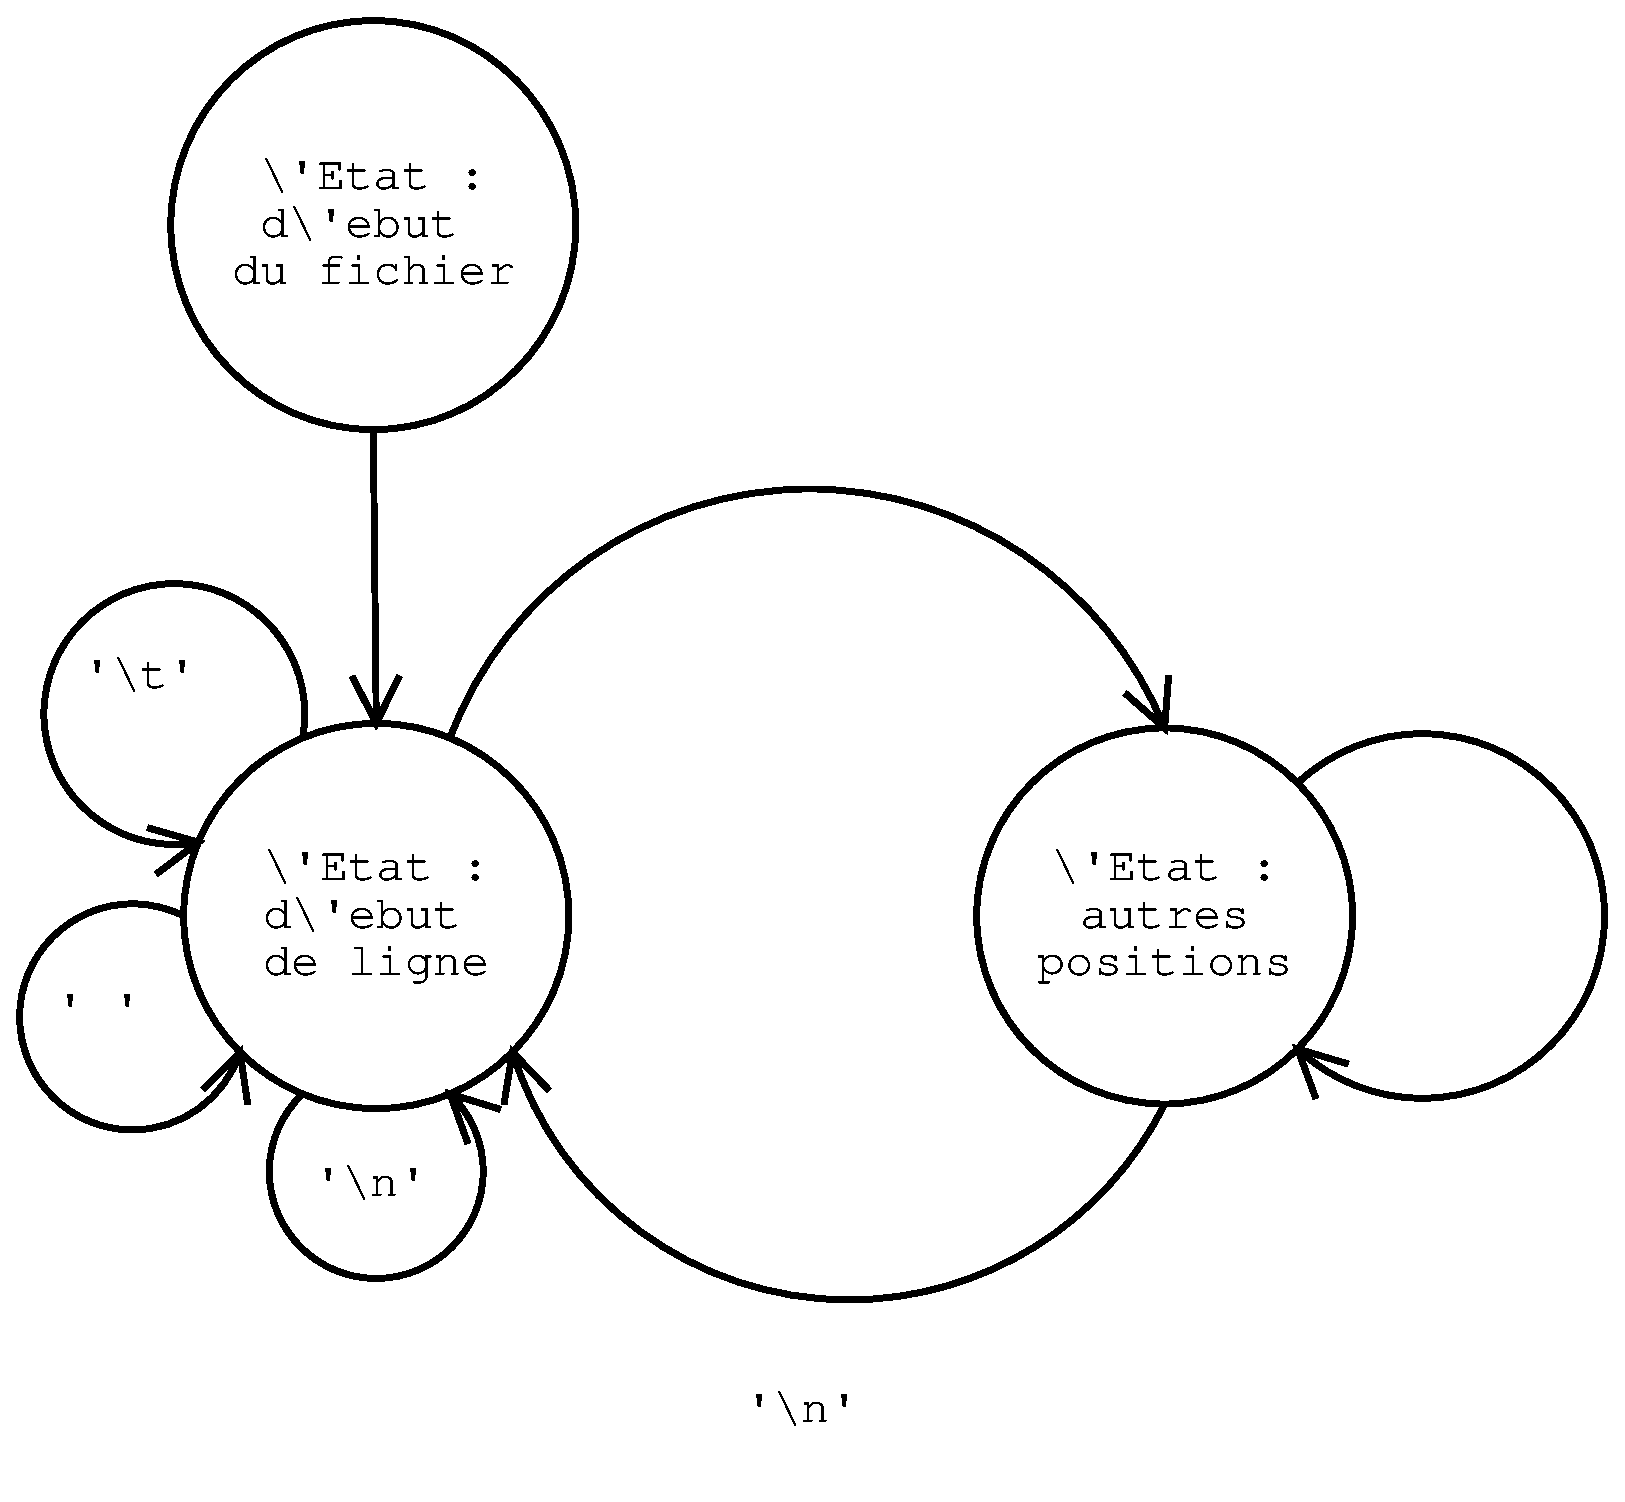
\includegraphics[scale=.3]{../Illustration/automatepp}  
%END LATEX
%HEVEA  \epsfbox{automatepp.ps}  
\end{center}
\begin{exercice}[Construction d'un programme \`a partir d'un automate]
  Inspirez vous de cet automate pour \'ecrire un filtre qui supprime
  les espaces ou les tabulations en d\'ebut de chaque ligne.
   \ifcorrection%
   \begin{correction}
\begin{verbatim}
     #include <stdio.h>
#include <stdlib.h>

int 
main()
{
    int c;
    enum {ETAT_DBT_LIGNE, ETAT_NORMAL } etat = ETAT_DBT_LIGNE;
  
    while ((c=getchar()) != EOF) {
        switch (etat) {
            case ETAT_DBT_LIGNE:
                switch (c) {
                    case ' ':
                    case '\t':
                        break;
                    default:   
                        putchar(c);
                        etat = ETAT_NORMAL;
                        break;
                }
                break;
            case ETAT_NORMAL:
                switch (c) {
                    case '\n': 
                        putchar('\n');
                        etat=ETAT_DBT_LIGNE;
                        break;
                    default :  
                        putchar(c);
                        break;
                }
        }
    }

    exit(EXIT_SUCCESS);
}
\end{verbatim}
   \end{correction}
   \fi%
\end{exercice}

\subsection{Le travail restant \`a faire}
Construisez l'automate codant nos r\`egles de styles et implantez le.
